%(Aquí lo dejaría con la estructura que teníamos para Caise, presentamos el framework y posteriormente comentamos modelos y transformaciones)

In this section we present $\pi$SOD-M, an MDD based methodology.
$\pi$SOD-M provides an environment for building service compositions considering
their non-functional requirements.
$\pi$SOD-M extends the SOD-M meta-models by adding
the concept of \textit{Policy}~\cite{Espinosa-Oviedo2011a}
to represent non-functional requirements.

\begin{figure}[h]
\centering
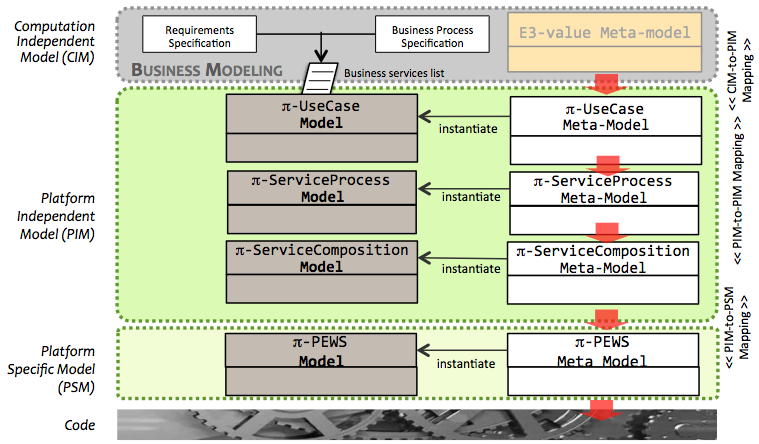
\includegraphics[width=1.0\textwidth]{figs/piSODM}
\caption{$\pi$SOD-M.}
\label{fig:piSOD-M}
\end{figure}

$\pi$SOD-M proposes the generation of a set of models at different abstraction levels, as
well as transformations between these models.
$\pi$SOD-M models represent both the functional aspects of the application as well as its non-functional constraints.
Constraints are restrictions that must be verified during the execution of the application.
An example of this is the requirement of the user's authentication for executing some system functions.

Similarly to SOD-M, our approach targets the construction of service-oriented applications that implement business processes.
$\pi$SOD-M proposes a development process based on the definition of models
(instances of the meta-modes) and transformations between models.
There are two kinds of transformations:
Model-to-model transformations are used during the software process to refine the specification.
Model-to-text transformations are the last step of the process and generate code.

We extended SOD-M to include non-functional specifications.
Our method defines four meta-models: \textit{$\pi$-UseCase}, \textit{$\pi$-ServiceProcess}, \textit{$\pi$-ServiceCom\-po\-si\-tion} and \textit{$\pi$-PEWS}.
The former three are extensions of SOD-M meta-models and belong to the PIM level.
The \textit{$\pi$-PEWS} meta-model is a PSM (Figure~\ref{fig:piSOD-M}).

The \textit{$\pi$-UseCase} meta-model describes functional and non-functional requirements.
Non-functional requirements are defined as \textit{constraints} over processing and data.
The \textit{$\pi$-ServiceProcess} meta-model defines the concept of \textit{service contract} to represent restrictions over data and actions that must be performed upon certain conditions.
The \textit{$\pi$-ServiceProcess} meta-model gathers the constraints
described in the \textit{$\pi$-UseCase} model into contracts that are associated
with services.
The \textit{$\pi$-ServiceComposition} meta-model provides the concept of \textit{Policy}
which put together contracts with similar non-functional requirements.
For instance, security and privacy restrictions may be grouped into a security policy.
\textit{$\pi$-ServiceComposition} models can be refined into PSMs.

At the PSM level we have lower-level models that can be automatically translated into actual computer programs.
The \textit{$\pi$-PEWS} meta-model is the PSM adopted in this work.
\textit{$\pi$-PEWS} models are textual descriptions of service compositions that can be translated into PEWS code~\cite{BaCAM05,Placido2010LTPD}.
Although PEWS is our language of choice, other composition languages can be used as target.
This can be accomplished by defining: \textit{(i)} a model-to-model transformation, from a \textit{$\pi$-ServiceComposition} model to the corresponding PSM, and \textit{(ii)} a model-to-text transformation, from the this PSM to the composition language.
